% =====================================================================
%  ME 697 -- Class Project: 1-D Lagrangian Hydrocode      Equation sheet v4
%  v4 (Oct 20): matches the code, bitwhiz f16485c (RS time loop 9d4ab24,
%  order 2 f16485c).  New Step 1, Face States (order = 1 or 2: MUSCL-
%  Hancock with a Van Leer limiter); later steps renumbered (Riemann
%  problem 2, positions 3, cell update 4); Where This Lives box now
%  describes the code as written.  Checked line by line against rs_mod
%  (rs_face_states, riemann_face, rs_cell_step, rs_state, rs_cell_dt)
%  and maincode (rs_region, section 6c).  Earlier notes follow.
%  v3 (Oct 20): the open decisions below settled by DK; zero-impedance
%  face and void-cell time step added.  v1/v2 notes follow.
%  v2 (Oct 19): Instructor's Note at the top (what bitwhiz is, the two
%  methods, AI assistance); text shared word for word with the AV sheet.
%  v1 notes follow.
%  Method RS (Riemann solver; Godunov's method, acoustic solver)
%  rev-0 draft, Oct 19, 2026 (with Claude).  Option B of the project.
%
%  Source of record: U7 (Acoustic Solution box), U3 (balance laws in h),
%  Kittell et al., PEP 45 (2020) 295-315, Sec. 2.3-2.4 (star-region values
%  stored at the faces; cells updated from their two faces), Toro (2009).
%  Open literature only.  Companion: Hydrocode_rev-1/Hydrocode_Eqns_v4
%  (Method AV, frozen) for the EOS, units, and the spall rule, shared.
%  Second order: van Leer, J. Comput. Phys. 32 (1979) (MUSCL, the limiter).
%
%  Through v3 this sheet was the DESIGN for bitwhiz's RS time loop; from
%  v4 it describes the code as written.  Decided (DK):
%    [1] Cell update: Godunov (conservative flux average), not random
%        choice (Oct 19).
%    [2] Time step per cell dx/c, no |u| (Lagrangian: waves move at +-Z in
%        h, and dh/Z = dx/c), times the same safety factor as AV: deck key
%        CFL, default 0.6 (Oct 20).  AV uses dx/(|ubar|+c).
%    [3] Ghost cells: P = Z = 0 and u = 0 (finite, so 0*u is 0, not NaN).
%    [4] A face with Z_L + Z_R = 0 (a void cell, c = 0, beside a ghost or
%        another void cell): P* = 0 and u* = the average of the two cell
%        velocities, a ghost taking its neighbor's (Oct 20).  Not reached
%        by the class materials.
%    [5] Total energy E = e + u^2/2 is updated; e = E - u^2/2 is stored
%        (slot je), as the EOS, spall rule and outputs need e (Oct 20).
%    [6] A void cell's time step (c = 0): dx/|u|, as in AV (in the code
%        since 9d4ab24).
%    [7] order = 1 | 2 (Solver block, RS only), default 2 = MUSCL-Hancock
%        with Van Leer, hard-coded; no user-chosen limiters (Oct 20).
%  Verified Oct 20, bitwhiz f16485c (Fortran), 2.00 km/s class problem,
%  35 zones/mm, CFL 0.6: order 1 reproduces the python prototype below to
%  1e-11 km/s in the PDV; release rms error against the reference (3.6 to
%  4.5 us): order 1 0.034, order 2 0.0045, AV 0.0054 km/s; energy
%  conserved to 1e-16 at both orders (notes: NOTES_bitwhiz_AV_vs_RS_v1).
%  Verified Oct 19 (python prototype of exactly these equations, bitwhiz's
%  EOS and spall rule, CFL 0.6, 35 zones/mm):
%    Al/Al symmetric impact, 1 km/s: plateau P = 8.2996 GPa vs 8.2983
%      analytic (+0.02%), u = 0.5000 km/s; energy and momentum conserved
%      to 2e-16 (relative) and 2e-15.
%    Double shock, 2.00 km/s, PDV (u* at MatX:PMMA): steps at 2.0433 and
%      2.3531 us (reference 2.0462, 2.3495), plateaus 1.5277 and 1.9700
%      km/s (reference 1.5278, 1.9695); bitwhiz AV 2.0445, 2.3526 us.
%      First order: the steps are smeared over a few more cells than AV.
% =====================================================================

\documentclass[11pt,addpoints]{exam}
\usepackage{amsfonts,amssymb,amsmath, amsthm}
\usepackage{graphicx}
\usepackage{enumitem}
\usepackage{systeme}
\usepackage{pgf,tikz,pgfplots}
\pgfplotsset{compat=1.15}
\usepgfplotslibrary{fillbetween}
\usepackage{mathrsfs}
\usepackage{multicol}
\usepackage{booktabs}
\usepackage[many]{tcolorbox}
\usepackage{bm}
\usepackage{cancel}

\allowdisplaybreaks

% Good Volume Symbol
\newcommand{\volume}{{\ooalign{$V$\cr\hfil\raisebox{0.35em}{\rule{2.1mm}{0.1ex}}\hfil\cr}}}

%%% Strike-out font
\usepackage{ulem}
\normalem
\pagestyle{headandfoot}

% ---- Warm theme to match the figures (U5 onward) ----
\definecolor{slate}{HTML}{2C3E50}
\definecolor{oiblue}{HTML}{0072B2}
\tcbset{colback=oiblue!4!white, colframe=slate, boxrule=0.5pt, arc=1.5mm}

\firstpageheader{ME 697 Equations}{Class Project: Hydrocode, Method RS}{Fall 2026 -- D. Kittell}
\runningheader{ME 697 Equations}{Class Project: Hydrocode, Method RS}{Fall 2026 -- D. Kittell}
\runningheadrule
\firstpagefooter{}{}{}
\runningfooter{}{}{}

\makeatletter
\renewcommand*\env@matrix[1][*\c@MaxMatrixCols c]{%
  \hskip -\arraycolsep
  \let\@ifnextchar\new@ifnextchar
  \array{#1}}
\makeatother

\begin{document}

\noindent
\bf{Instructor's Note:}\normalfont\\

\noindent
\it{\texttt{bitwhiz} is the reference hydrocode for ME 697, Intermediate Shock and Detonation Theory (Purdue, Fall 2026): a one-dimensional, planar, Lagrangian code for plate impact, with shock and release waves crossing layers of solids and liquids, and spall where release waves meet in tension. Two solution methods share one code: this sheet is Method RS (a Riemann solver), and the companion sheet is Method AV (artificial viscosity). It was written by D.~Kittell with the assistance of Claude Opus 5.5 (Anthropic), an AI model; the instructor directed, reviewed, and tested every part of it and is responsible for its content.}\normalfont\vspace{1.5em}

\textbf{These equations build upon U3. Continuum Mechanics {\&} Balance Laws, U7. The Riemann Problem for Compressible Fluids (Acoustic Solution), and the Method AV sheet (units, equation of state, spall)}\vspace{1em}

\begin{tcolorbox}[breakable]
\textbf{Notation \& Scope:}\vspace{.5em}
\begin{itemize}
\item One-dimensional hydrocode, planar, Lagrangian, and purely hydrodynamic, such that \hspace{3mm} \bm{$\sigma_{xx}\;=\;-P$} \hspace{5mm} with \bm{$Y=0$} and \textbf{\emph{no artificial viscosity}}\vspace{.5em}
\item Cell-Centered Grid, \hspace{3mm} \bm{$\rho$}, \bm{$\text{V}=1/\rho$}, \bm{$u$}, \bm{$e$}, \bm{$E=e+\frac{1}{2}u^2$}, \bm{$P$}, \bm{$c$}, \bm{$Z=\rho c$} \hspace{2mm} live in the cells, \textbf{\emph{velocity included}}; \hspace{3mm} a face carries its position \bm{$x$} and the Riemann solution \bm{$u_\star$}, \bm{$P_\star$}\vspace{.5em}
\item Indices, \hspace{3mm} cells \bm{$k$}, faces \bm{$k\pm\frac{1}{2}$}; \hspace{2mm} the cell state is at whole steps \bm{$n$}; \hspace{2mm} \bm{$u_\star$} and \bm{$P_\star$} hold for the whole step \bm{$n\rightarrow n+1$}, so they carry \bm{$n+\frac{1}{2}$}\vspace{.5em}
\item Face States, \hspace{3mm} \bm{$u^L_k$}, \bm{$P^L_k$} and \bm{$u^R_k$}, \bm{$P^R_k$}: what cell \bm{$k$} offers the Riemann problems on its left (\bm{$k-\frac{1}{2}$}) and right (\bm{$k+\frac{1}{2}$}) faces (Step 1)\vspace{.5em}
\item Cell Mass, \hspace{3mm} \bm{$M_k$} \hspace{2mm} per unit area, fixed; \hspace{2mm} the areal mass coordinate \bm{$h$} of U7 advances by \bm{$M_k$} per cell, and faces are lines \bm{$h=$} const.\vspace{.5em}
\item Star Region, \hspace{3mm} \bm{$u_\star$} and \bm{$P_\star$} are continuous across the contact (U7); \bm{$\text{V}_{\star L}$} and \bm{$\text{V}_{\star R}$} are not, and this method never needs them\vspace{.5em}
\item Boxes titled \textbf{bitwhiz:} go beyond the \textbf{\emph{project rules}}, to what the reference code \texttt{bitwhiz} does (deck: \texttt{method = RS})
\end{itemize}
\end{tcolorbox}

\clearpage

\begin{tcolorbox}[breakable]
\textbf{Units and Shared Pieces (from the Method AV sheet):}\vspace{.5em}
\begin{itemize}
\item Units, \hspace{3mm} \bm{$x$} [mm], \hspace{2mm} \bm{$t$} [\bm{$\mu$}s], \hspace{2mm} \bm{$\rho$} [g/cm\bm{$^3$}], \hspace{2mm} \bm{$u,\;c$} [km/s], \hspace{2mm} \bm{$P$} [GPa], \hspace{2mm} \bm{$e$} [MJ/kg], \hspace{2mm} \bm{$M_k$} [g/cm\bm{$^3\cdot$}mm], \hspace{2mm} \bm{$Z$} [g/cm\bm{$^3\cdot$}km/s] \hspace{2mm} so \bm{$Z\,u$} [GPa]\vspace{.5em}
\item Shared, \hspace{3mm} the mesh of Step 0, the equation of state \bm{$P\left(\rho,e\right)$} and sound speed \bm{$c$}, the void boundary, and (\texttt{bitwhiz}) the spall rule and expansion branch: \textbf{\emph{the same as Method AV}}
\end{itemize}
\end{tcolorbox}

\;\\

\begin{tcolorbox}[breakable]
\textbf{Godunov's Method, and Its Relatives (a Map, Not a Recipe):}\vspace{.5em}
\begin{itemize}
\item Godunov (1959), \hspace{3mm} keep one \textbf{\emph{average}} state per cell; at every face, solve the Riemann problem between the two neighbor cells; use its solution as the \textbf{\emph{flux}} through that face for one step; update each cell from its two faces. Conservative, monotone, first order; shocks are captured without \bm{$q$}, smeared over a few cells\vspace{.5em}
\item The Riemann Solver, \hspace{3mm} \textbf{\emph{what goes at the face}}: \hspace{2mm} exact (iterative, U7); \hspace{2mm} \textbf{acoustic} (this sheet: \bm{$Z$} frozen for one step, no iteration); \hspace{2mm} HLL/HLLC (estimated wave speeds; in \bm{$h$} with speeds \bm{$-Z_L$}, \bm{$+Z_R$}, the HLLC star state \textbf{\emph{is}} the acoustic one); \hspace{2mm} two-shock (Dukowicz 1985: \bm{$Z\approx\rho\left(c+s_1\left|u_\star-u\right|\right)$}, a shock impedance from \bm{$U_S$}--\bm{$u_p$} data)\vspace{.5em}
\item Reconstruction, \hspace{3mm} \textbf{\emph{what states the face sees}}: \hspace{2mm} first order uses the cell averages; \hspace{2mm} MUSCL (van Leer 1979, first written for Lagrangian gas dynamics) puts a limited linear slope in each cell, second order; \hspace{2mm} WENO5 blends three quadratics, fifth order where smooth. Both sharpen shocks; in general both need two ghost cells per end (\texttt{bitwhiz}'s order 2 is MUSCL-Hancock with Van Leer's limiter, Step 1)\vspace{.5em}
\item Time Integration, \hspace{3mm} first order is forward Euler with the face fluxes held over the step; with MUSCL, use a MUSCL-Hancock half step or a strong-stability-preserving Runge-Kutta (RK2/RK3) so the time order matches the space order\vspace{.5em}
\item Splitting, \hspace{3mm} Strang splitting combines separate operators (hydro, then a reaction or a second direction) to second order; one-dimensional inert hydro needs none\vspace{.5em}
\item References, \hspace{3mm} Godunov, \emph{Mat.\ Sb.}\ \textbf{47} (1959); \hspace{1mm} van Leer, \emph{J.\ Comput.\ Phys.}\ \textbf{32} (1979); \hspace{1mm} Dukowicz, \emph{J.\ Comput.\ Phys.}\ \textbf{61} (1985); \hspace{1mm} Toro, \emph{Riemann Solvers and Numerical Methods for Fluid Dynamics} (Springer, 2009); \hspace{1mm} Kittell et al., \emph{Propellants Explos.\ Pyrotech.}\ \textbf{45} (2020) 295--315
\end{itemize}
\end{tcolorbox}

\clearpage

\begin{tcolorbox}[breakable]
\textbf{Step 0. Mesh and Initial Conditions:}\vspace{.5em}
\begin{itemize}
\item Faces and Cell Mass, \hspace{3mm} as in Method AV: \textbf{\emph{every material interface lands on a cell face}}, \hspace{2mm} \bm{$\displaystyle M_k\;=\;\rho_{0,k}\left(x^0_{k+\frac{1}{2}}-x^0_{k-\frac{1}{2}}\right)$}\vspace{.5em}
\item Cell State, \hspace{3mm} \bm{$\rho^0_k=\rho_{0,k}$}, \hspace{2mm} \bm{$e^0_k=0$}, \hspace{2mm} \bm{$P^0_k=0$}, \hspace{2mm} \bm{$c^0_k=c_{0,k}$}, \hspace{2mm} \bm{$u^0_k=u_{0,k}$} \hspace{7mm} the cell's own initial velocity\vspace{.5em}
\item Impact Face, \hspace{3mm} nothing special: two cells with different velocities meet at a face, which \textbf{\emph{is}} a Riemann problem; no momentum-weighted starting value is needed
\end{itemize}
\end{tcolorbox}

\;\\

\begin{tcolorbox}[breakable]
\textbf{Step 1. Face States, What Each Cell Offers Its Faces (\texttt{order} = 1 or 2):}\vspace{.5em}
\begin{itemize}
\item Order 1, \hspace{3mm} (the project's Option B) \hspace{3mm} \bm{$u^L_k=u^R_k=u^n_k$}, \hspace{3mm} \bm{$P^L_k=P^R_k=P^n_k$} \hspace{7mm} the cell averages: first-order Godunov\vspace{.5em}
\item Order 2 (\texttt{bitwhiz}, the default), \hspace{3mm} MUSCL-Hancock. For \bm{$W=u$} and \bm{$W=P$}, the slopes per unit mass to each neighbor\vspace{.5em}\\
.~~~~~~~~~~\bm{$\displaystyle a\;=\;\frac{W_k-W_{k-1}}{\frac{1}{2}\left(M_{k-1}+M_k\right)}$} \hspace{9mm} \bm{$\displaystyle b\;=\;\frac{W_{k+1}-W_k}{\frac{1}{2}\left(M_k+M_{k+1}\right)}$} \hspace{7mm} all at \bm{$n$}\vspace{1em}
\item Van Leer Limiter, \hspace{3mm} \bm{$\displaystyle s_W\;=\;\frac{2ab}{a+b}$} \hspace{2mm} if \bm{$ab>0$}, \hspace{2mm} else \bm{$s_W=0$} \hspace{7mm} a peak or trough gets no slope, so no new extremum (no ringing)\vspace{.5em}
\item Half Step, \hspace{3mm} each face value advanced by \bm{$\frac{1}{2}\Delta t^n$} with the cell's own acoustic equations, \hspace{2mm} \bm{$\partial u/\partial t=-\partial P/\partial h$}, \hspace{2mm} \bm{$\partial P/\partial t=-Z^2\,\partial u/\partial h$}\vspace{.5em}\\
.~~~~~~~~~~\bm{$\displaystyle u^{L,R}_k\;=\;u^n_k\;\mp\;\frac{M_k}{2}s_u\;-\;\frac{\Delta t^n}{2}\,s_P$}\vspace{1em}\\
.~~~~~~~~~~\bm{$\displaystyle P^{L,R}_k\;=\;P^n_k\;\mp\;\frac{M_k}{2}s_P\;-\;\frac{\Delta t^n}{2}\left(Z^n_k\right)^2s_u$}\vspace{1em}
\item Only \bm{$u$} and \bm{$P$}, \hspace{3mm} the acoustic solver takes \bm{$Z$} from the cell averages, and \bm{$u$}, \bm{$P$} are continuous across a material interface, so a slope may span one; \bm{$\text{V}$}, which jumps there, is never reconstructed\vspace{.5em}
\item Ends, \hspace{3mm} a cell beside a ghost gets \bm{$s_u=s_P=0$}: the free surfaces stay first order, and one ghost cell per end is enough
\end{itemize}
\end{tcolorbox}

\clearpage

\begin{figure}[!ht]
  \centering
  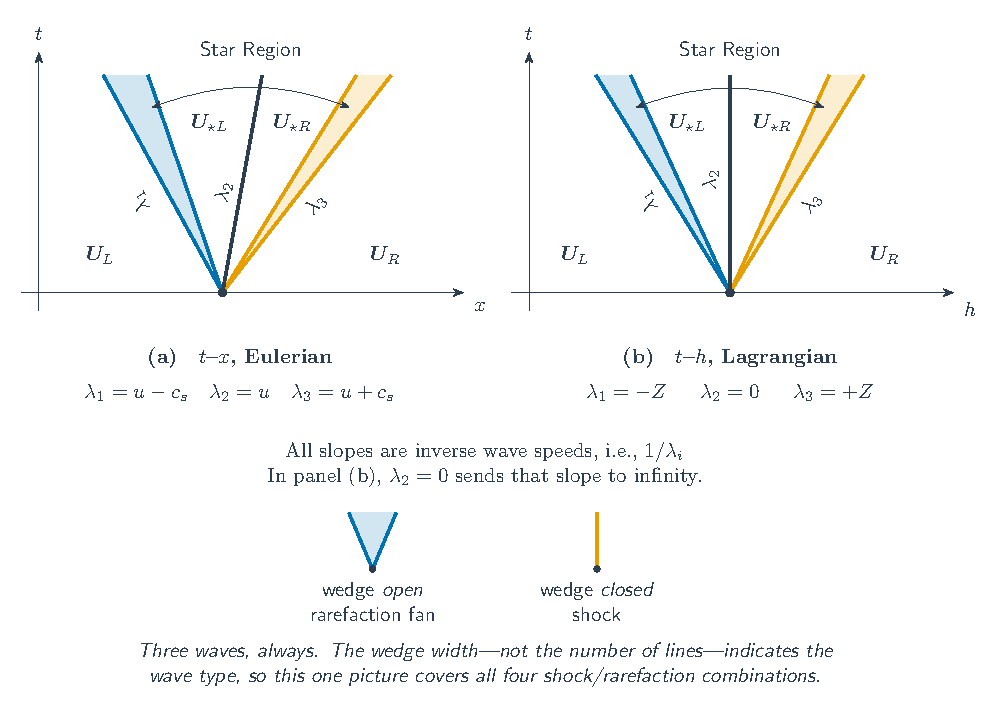
\includegraphics[width=0.56\textwidth]{riemann_schematic_v5.pdf}
  \caption{The Riemann problem at one face (from U7; representational only). In the Lagrangian frame (b) the face is the line \bm{$h=$} const.; the left and right waves leave it at \bm{$-Z_L$} and \bm{$+Z_R$}, and the face itself carries \bm{$u_\star$} and \bm{$P_\star$}.\label{fig:rp}}
\end{figure}

\begin{tcolorbox}[breakable]
\textbf{Step 2. The Riemann Problem at Every Face (Acoustic Solution, U7):}\vspace{.5em}
\begin{itemize}
\item Left and Right, \hspace{3mm} for the face \bm{$k+\frac{1}{2}$}: \hspace{2mm} \bm{$u_L=u^R_k$}, \bm{$P_L=P^R_k$} \hspace{2mm} from cell \bm{$k$}, \hspace{2mm} \bm{$u_R=u^L_{k+1}$}, \bm{$P_R=P^L_{k+1}$} \hspace{2mm} from cell \bm{$k+1$} (Step 1); \hspace{3mm} impedances \hspace{2mm} \bm{$Z_L=\rho^n_kc^n_k$}, \hspace{2mm} \bm{$Z_R=\rho^n_{k+1}c^n_{k+1}$}, \hspace{2mm} held fixed for the step\vspace{.5em}
\item Riemann Invariants, \hspace{3mm} \bm{$\displaystyle \Phi_1\;=\;P_L\;+\;Z_Lu_L$} \hspace{7mm} \bm{$\displaystyle \Phi_2\;=\;P_R\;-\;Z_Ru_R$}\vspace{.5em}
\item Star State, \hspace{3mm} \bm{$\displaystyle u^{n+\frac{1}{2}}_{\star,k+\frac{1}{2}}\;=\;\frac{\Phi_1\;-\;\Phi_2}{Z_L\;+\;Z_R}$} \hspace{9mm} \bm{$\displaystyle P^{n+\frac{1}{2}}_{\star,k+\frac{1}{2}}\;=\;\frac{Z_R\Phi_1\;+\;Z_L\Phi_2}{Z_L\;+\;Z_R}$}\vspace{1em}
\item Expanded, \hspace{3mm} \bm{$\displaystyle u_\star\;=\;\frac{Z_Lu_L\;+\;Z_Ru_R\;+\;P_L\;-\;P_R}{Z_L\;+\;Z_R}$}\vspace{1em}\\
.~~~~~~~~~~~~~~~~~~~~~~~\bm{$\displaystyle P_\star\;=\;\frac{Z_RP_L\;+\;Z_LP_R\;+\;Z_LZ_R\left(u_L-u_R\right)}{Z_L\;+\;Z_R}$}\vspace{1em}
\item Reading \bm{$P_\star$}, \hspace{3mm} for \bm{$Z_L=Z_R=Z$}: \hspace{2mm} \bm{$\displaystyle P_\star\;=\;\frac{P_L+P_R}{2}\;+\;\frac{Z}{2}\left(u_L-u_R\right)$} \hspace{7mm} the average, plus a \textbf{\emph{built-in viscosity}} \bm{$\propto\rho c\,\Delta u$}\vspace{.5em}
\item Impact Check, \hspace{3mm} \bm{$P_L=P_R=0$}, \hspace{2mm} \bm{$u_R=0$}: \hspace{2mm} \bm{$\displaystyle u_\star=\frac{Z_Lu_L}{Z_L+Z_R}$}, \hspace{2mm} \bm{$\displaystyle P_\star=\frac{Z_LZ_Ru_L}{Z_L+Z_R}$} \hspace{7mm} the U6 impedance match, with acoustic \bm{$Z$}\vspace{.5em}
\item Note: frozen \bm{$Z$} is a weak-wave approximation \textbf{\emph{at one face for one step}}; the shock speed and jump still come out right, because Steps 3--4 conserve mass, momentum, and energy exactly
\end{itemize}
\end{tcolorbox}

\;\\

\begin{tcolorbox}[breakable]
\textbf{Step 3. Positions and Densities:}\vspace{.5em}
\begin{itemize}
\item Face Motion, \hspace{3mm} \bm{$\displaystyle x^{n+1}_{k+\frac{1}{2}}\;=\;x^n_{k+\frac{1}{2}}\;+\;u^{n+\frac{1}{2}}_{\star,k+\frac{1}{2}}\,\Delta t^n$} \hspace{7mm} the face moves with the contact\vspace{.5em}
\item Cell Density, \hspace{3mm} \bm{$\displaystyle \rho^{n+1}_k\;=\;\frac{M_k}{x^{n+1}_{k+\frac{1}{2}}\;-\;x^{n+1}_{k-\frac{1}{2}}}$} \hspace{7mm} identical to the volume flux update \hspace{2mm} \bm{$\displaystyle \text{V}^{n+1}_k=\text{V}^n_k+\frac{\Delta t^n}{M_k}\left(u_{\star,k+\frac{1}{2}}-u_{\star,k-\frac{1}{2}}\right)$}
\end{itemize}
\end{tcolorbox}

\;\\

\begin{tcolorbox}[breakable]
\textbf{Step 4. Velocity, Energy, and Pressure (Each Cell from Its Two Faces):}\vspace{.5em}
\begin{itemize}
\item Momentum, \hspace{3mm} \bm{$\displaystyle u^{n+1}_k\;=\;u^n_k\;-\;\frac{\Delta t^n}{M_k}\left(P_{\star,k+\frac{1}{2}}\;-\;P_{\star,k-\frac{1}{2}}\right)$}\vspace{.5em}
\item Total Energy, \hspace{3mm} \bm{$\displaystyle E^{n+1}_k\;=\;E^n_k\;-\;\frac{\Delta t^n}{M_k}\left[\left(P_\star u_\star\right)_{k+\frac{1}{2}}\;-\;\left(P_\star u_\star\right)_{k-\frac{1}{2}}\right]$}\vspace{.5em}
\item Internal Energy, \hspace{3mm} \bm{$\displaystyle e^{n+1}_k\;=\;E^{n+1}_k\;-\;\frac{1}{2}\left(u^{n+1}_k\right)^2$}\vspace{.5em}
\item Pressure and Sound Speed, \hspace{3mm} \bm{$P^{n+1}_k=P\left(\rho^{n+1}_k,e^{n+1}_k\right)$}, \hspace{2mm} kept \bm{$\ge 0$} (\texttt{bitwhiz}: the spall rule), \hspace{2mm} then \bm{$c^{n+1}_k$} at the pressure kept \hspace{7mm} as in Method AV\vspace{.5em}
\item Conservation, \hspace{3mm} each face flux leaves one cell and enters its neighbor, so the sums telescope: total mass, momentum \bm{$\sum M_ku_k$}, and energy \bm{$\sum M_kE_k$} are conserved \textbf{\emph{to round-off}} (\bm{$P_\star=0$} at both free surfaces)
\end{itemize}
\end{tcolorbox}

\clearpage

\begin{tcolorbox}[breakable]
\textbf{Time Step (CFL Condition):}\vspace{.5em}
\begin{itemize}
\item Per Cell, \hspace{3mm} \bm{$\displaystyle \Delta t_k\;=\;\frac{x^{n+1}_{k+\frac{1}{2}}\;-\;x^{n+1}_{k-\frac{1}{2}}}{c^{n+1}_k}\;=\;\frac{M_k}{Z^{n+1}_k}$} \hspace{7mm} in \bm{$h$} the waves move at \bm{$\pm Z$}; no \bm{$\left|u\right|$}, the mesh moves with it\vspace{.5em}
\item CFL Criterion, \hspace{3mm} \bm{$\displaystyle \Delta t^{n+1}\;=\;\text{CFL}\;\min_k\left(\Delta t_k\right)$}, \hspace{2mm} \bm{$\text{CFL}=0.6$} \hspace{7mm} a safety factor, as in Method AV (\texttt{bitwhiz}: deck key \texttt{CFL}, default 0.6)\vspace{.5em}
\item Why \bm{$\text{CFL}\le 1$}, \hspace{3mm} no wave crosses a cell within a step, so neighboring Riemann problems never meet and the frozen \bm{$Z$} of Step 2 stays valid; the order 2 half step (Step 1) is stable under the same limit\vspace{.5em}
\item Void Cell (\texttt{bitwhiz}), \hspace{3mm} \bm{$c=0$}: \hspace{2mm} \bm{$\displaystyle \Delta t_k=\frac{\Delta x}{\left|u_k\right|}$}, as in Method AV (no limit if it is at rest)\vspace{.5em}
\item First and Last Steps, \hspace{3mm} \bm{$\Delta t^0$} from the \bm{$t=0$} state (\bm{$c=c_0$}); \hspace{2mm} the last step is shortened to land exactly on the termination time
\end{itemize}
\end{tcolorbox}

\;\\

\begin{tcolorbox}[breakable]
\textbf{Boundary Conditions (Void on Both Ends):}\vspace{.5em}
\begin{itemize}
\item Ghost Cells, \hspace{3mm} \bm{$k=0$} \hspace{2mm} and \hspace{2mm} \bm{$k=k_{\max}+1$} \hspace{5mm} with \hspace{2mm} \bm{$P=0$}, \hspace{2mm} \bm{$Z=0$}, \hspace{2mm} \bm{$u=0$} \hspace{2mm} (any finite value; it is multiplied by \bm{$Z=0$})\vspace{.5em}
\item Effect, \hspace{3mm} the Step 2 formulas, with nothing changed, give at the left end (\bm{$Z_L=0$}; no slope beside a ghost, so \bm{$u^L_1=u_1$}, \bm{$P^L_1=P_1$})\vspace{.5em}\\
.~~~~~~~~~~\bm{$\displaystyle u_{\star,\frac{1}{2}}\;=\;u_1\;-\;\frac{P_1}{Z_1}$} \hspace{9mm} \bm{$\displaystyle P_{\star,\frac{1}{2}}\;=\;0$} \hspace{9mm} the acoustic \textbf{\emph{free surface}} (velocity doubling for a shocked state)\vspace{1em}
\item Interfaces, \hspace{3mm} nothing special: each side brings its own \bm{$Z$}, and each cell calls its own EOS\vspace{.5em}
\item Zero Impedance (\texttt{bitwhiz}), \hspace{3mm} if \bm{$Z_L+Z_R=0$} (a void cell, \bm{$c=0$}, beside a ghost or another void cell): \hspace{2mm} \bm{$P_\star=0$} \hspace{2mm} and \hspace{2mm} \bm{$u_\star=\frac{1}{2}\left(u_L+u_R\right)$}, a ghost taking its neighbor's face \bm{$u$} \hspace{7mm} not reached by the class materials
\end{itemize}
\end{tcolorbox}

\clearpage

\begin{tcolorbox}[breakable]
\textbf{One Cycle, In Order:}\vspace{.5em}
\begin{itemize}
\item[a.] Face states \bm{$u^{L,R}$}, \bm{$P^{L,R}$} in every cell (order 1: the cell values; order 2: slopes and half step)
\item[b.] Riemann solution \bm{$u_\star$}, \bm{$P_\star$} on every face, with \bm{$Z^n=\rho^nc^n$} from its two cells
\item[c.] Positions \bm{$x^{n+1}$}, then densities \bm{$\rho^{n+1}$}
\item[d.] Velocities \bm{$u^{n+1}$} and total energies \bm{$E^{n+1}$}, then \bm{$e^{n+1}$}
\item[e.] Pressures \bm{$P^{n+1}$} (keep them \bm{$\ge 0$}; \texttt{bitwhiz}: the spall rule), then sound speeds \bm{$c^{n+1}$}
\item[f.] The next time step \bm{$\Delta t^{n+1}$}
\item[g.] Write output if needed; \bm{$n\leftarrow n+1$}; repeat until the termination time\vspace{.5em}
\item Compared with Method AV, \hspace{3mm} no \bm{$q$}, no node mass, no half-step velocity, no kinetic-energy correction: the Riemann solution at the face replaces all four
\end{itemize}
\end{tcolorbox}

\;\\

\begin{tcolorbox}[breakable]
\textbf{bitwhiz: Where This Lives in the Code:}\vspace{.5em}
\begin{itemize}
\item Deck, \hspace{3mm} \texttt{method = RS} \hspace{2mm} and, optionally, \hspace{2mm} \texttt{order = 1} or \texttt{2} (default 2) in the Solver block; \hspace{2mm} every output names the scheme, e.g.\ ``RS, order 2 (MUSCL-Hancock, Van Leer)''\vspace{.5em}
\item Steps, \hspace{3mm} module \texttt{rs}: \hspace{2mm} Step 1 \bm{$\rightarrow$} \texttt{rs\_face\_states}; \hspace{2mm} Step 2 \bm{$\rightarrow$} \texttt{riemann\_face}; \hspace{2mm} Steps 3--4 \bm{$\rightarrow$} \texttt{rs\_cell\_step} (\bm{$\rho$}, \bm{$u$}, \bm{$E$}, \bm{$e$}) and \texttt{rs\_state} (EOS, spall rule and \bm{$c$}, through \texttt{cell\_pressure}, shared with Method AV); \hspace{2mm} Time Step \bm{$\rightarrow$} \texttt{rs\_cell\_dt}\vspace{.5em}
\item One Cycle, \hspace{3mm} \texttt{maincode}, contained routine \texttt{rs\_region}: loop 0, cells (a); loop 1, faces (b, and \bm{$x^{n+1}$}); loop 2, cells (\bm{$\rho^{n+1}$}, then d--f); one OpenMP parallel region, as for AV, and the same answer on any number of threads\vspace{.5em}
\item Database Slots, \hspace{3mm} faces: \bm{$x$} \texttt{jx}, \hspace{1mm} \bm{$u_\star$} \texttt{ju\_star}, \hspace{1mm} \bm{$P_\star$} \texttt{jp\_star}; \hspace{3mm} cells: \bm{$M_k$} \texttt{jm}, \hspace{1mm} \bm{$\rho$} \texttt{jrho}, \hspace{1mm} \bm{$u$} \texttt{juc}, \hspace{1mm} \bm{$e$} \texttt{je}, \hspace{1mm} \bm{$P$} \texttt{jp}, \hspace{1mm} \bm{$c$} \texttt{jc}, \hspace{1mm} \bm{$\mathcal{D}$} \texttt{jdam}, \hspace{1mm} \bm{$u^L,u^R,P^L,P^R$} \texttt{ju\_lf}, \texttt{ju\_rf}, \texttt{jp\_lf}, \texttt{jp\_rf}, and the material constants; \hspace{2mm} \bm{$Z=\rho c$} is formed on the spot, not stored\vspace{.5em}
\item Outputs, \hspace{3mm} the tracer column \texttt{KMPS} is \bm{$u_\star$}; \texttt{Q} is NaN (there is no \bm{$q$}); the PDV tracer on an interface face reads \bm{$u_\star$} there
\end{itemize}
\end{tcolorbox}

\end{document}
